\documentclass[12pt, letterpaper]{article}

% --- PAQUETES ---
\usepackage[utf8]{inputenc}
\usepackage[spanish]{babel}
\usepackage{amsmath}
\usepackage{amssymb}
\usepackage{geometry}
\usepackage{graphicx}

% --- CONFIGURACIÓN DE PÁGINA ---
\geometry{letterpaper, margin=1in}



% --- INICIO DEL DOCUMENTO ---
\begin{document}


\section*{Resolución de los ejercicios}
\section*{1.}
\subsection*{a) Ecuación de la recta tangente}
\textbf{Problema:} Determine la ecuación de la recta tangente a la curva $y = \ln(x^2 - 3x + 1)$ en el punto $(3,0)$.

\subsubsection*{Solución}
Para encontrar la ecuación de la recta tangente, se siguen los siguientes pasos:

\paragraph{1. Calcular la derivada de la función.}
Se utiliza la regla de la cadena para derivar la función $y$ con respecto a $x$:
$$
\frac{dy}{dx} = \frac{d}{dx} \left( \ln(x^2 - 3x + 1) \right)
$$
La derivada es:
$$
\frac{dy}{dx} = \frac{1}{x^2 - 3x + 1} \cdot (2x - 3) = \frac{2x - 3}{x^2 - 3x + 1}
$$

\paragraph{2. Calcular la pendiente ($m$) en el punto de tangencia.}
Se evalúa la derivada en la coordenada $x$ del punto dado, es decir, $x=3$:
$$
m = \frac{dy}{dx}\bigg|_{x=3} = \frac{2(3) - 3}{(3)^2 - 3(3) + 1} = \frac{6 - 3}{9 - 9 + 1} = \frac{3}{1} = 3
$$

\paragraph{3. Determinar la ecuación de la recta.}
Se utiliza la forma punto-pendiente de la ecuación de una recta, $y - y_1 = m(x - x_1)$, con el punto $(x_1, y_1) = (3,0)$ y la pendiente encontrada anteriormente $m=3$:
$$
y - 0 = 3(x - 3)
$$
Simplificamos la expresión y obtenemos la ecuación de la recta tangente al punto que deseamos:
$$
\mathbf{y = 3x - 9}
$$

\subsection*{Gráfica de las funciones}
\begin{figure}[h]
    \centering
    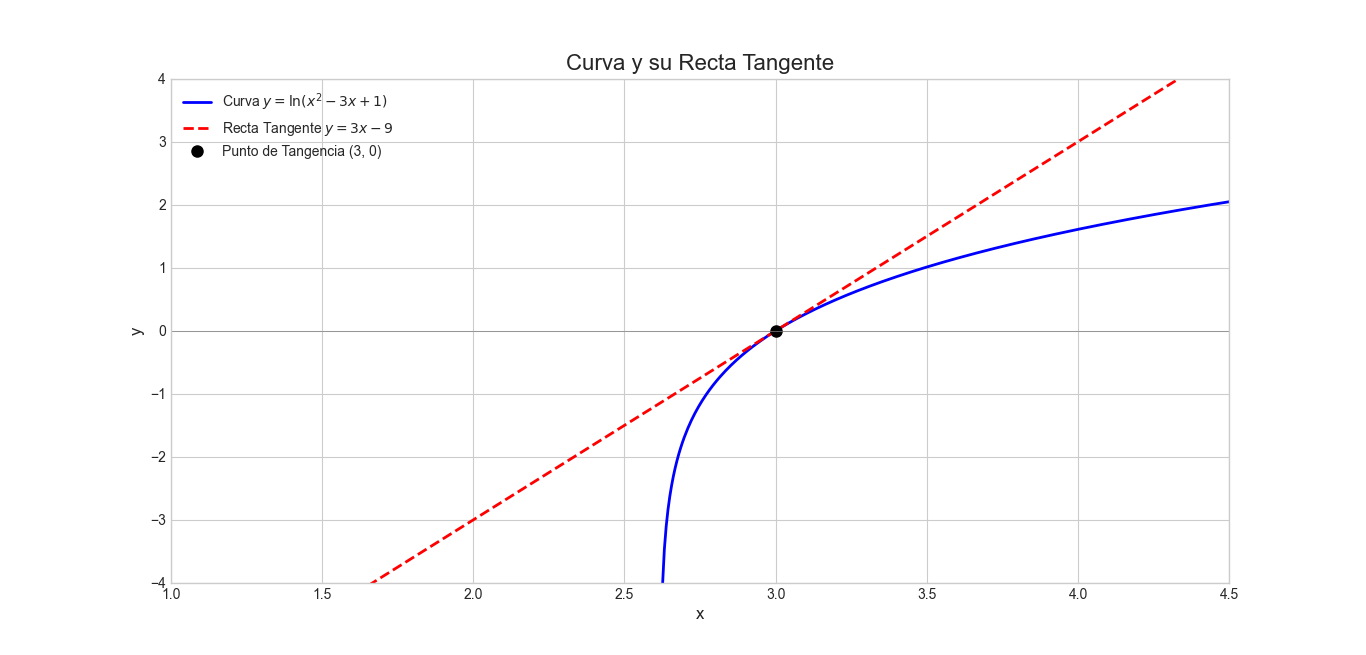
\includegraphics[width=0.75\textwidth]{Figure_2.png}
    \caption{Derivada, Recta y Punto de tangencia}
    \label{fig:Figure_2}
\end{figure}

\newpage
\subsection*{b) Derivación logarítmica}
\textbf{Problema:} Utilice la derivación logarítmica para hallar $y'$ si $x^y = y^x$.

\subsubsection*{Solución}
Para hallar la derivada $\frac{dy}{dx}$, se aplica el método de derivación logarítmica: ( Según la sección 3.6, pagina 220. Stewart, 8va edición.)

\paragraph{1. Aplicar logaritmo natural.}
Se toma el logaritmo natural en ambos lados de la ecuación original:
$$
\ln(x^y) = \ln(y^x)
$$
Aplicando la propiedad de los logaritmos $\ln(a^b) = b\ln(a)$, la ecuación se convierte en:
$$
y \ln(x) = x \ln(y)
$$

\paragraph{2. Derivar implícitamente con respecto a $x$.}
Se deriva cada lado de la ecuación, aplicando la regla del producto:
$$
\frac{d}{dx}(y \ln(x)) = \frac{d}{dx}(x \ln(y))
$$
$$
\frac{dy}{dx} \cdot \ln(x) + y \cdot \frac{1}{x} = 1 \cdot \ln(y) + x \cdot \frac{1}{y} \cdot \frac{dy}{dx}
$$

\paragraph{3. Agrupamos $\frac{dy}{dx}$.}
Se agrupan todos los términos que contienen $\frac{dy}{dx}$ en un lado de la ecuación:
$$
\frac{dy}{dx} \ln(x) - \frac{x}{y} \frac{dy}{dx} = \ln(y) - \frac{y}{x}
$$
Se factoriza $\frac{dy}{dx}$:
$$
\frac{dy}{dx} \left( \ln(x) - \frac{x}{y} \right) = \ln(y) - \frac{y}{x}
$$
Finalmente, se resuelve para $\frac{dy}{dx}$:
$$
\frac{dy}{dx} = \frac{\ln(y) - \frac{y}{x}}{\ln(x) - \frac{x}{y}}
$$

\paragraph{4. Simplificamos}

$$
\frac{dy}{dx} = \frac{\frac{x\ln(y) - y}{x}}{\frac{y\ln(x) - x}{y}} = \frac{y(x\ln(y) - y)}{x(y\ln(x) - x)}
$$
La derivada es:
$$
\mathbf{\frac{dy}{dx} = \frac{y(x\ln(y) - y)}{x(y\ln(x) - x)}}
$$

\section*{2.}

La Ley de Boyle establece la relación entre la presión ($P$) y el volumen ($V$) de una muestra de gas a temperatura constante mediante la ecuación:
$$
PV = C
$$
donde $C$ es una constante.

\subsection*{Datos del Problema}
Se nos proporcionan los siguientes datos para un instante específico:
\begin{itemize}
    \item Volumen actual ($V$): $600 \text{ cm}^3$
    \item Presión actual ($P$): $150 \text{ kPa}$
    \item Razón de cambio de la presión ($\frac{dP}{dt}$): $+20 \text{ kPa/min}$ 
\end{itemize}

\subsection*{Objetivo}
Se busca determinar la razón con la que el volumen del gas disminuye en ese mismo instante, es decir, encontrar el valor de $\frac{dV}{dt}$.

\subsection*{Solución}

\paragraph{1. Calcular la constante C.}
$$
C = P \cdot V = (150 \text{ kPa}) \cdot (600 \text{ cm}^3) = 90000 \text{ kPa} \cdot \text{cm}^3
$$

\paragraph{2. Diferenciar la Ley de Boyle con respecto al tiempo (t).}
Para encontrar la relación entre las razones de cambio, derivamos la ecuación $PV = C$ de forma implícita.
$$
\frac{d}{dt}(PV) = \frac{d}{dt}(C)
$$
$$
\frac{dP}{dt} \cdot V + P \cdot \frac{dV}{dt} = 0
$$

\paragraph{3. Sustituir los valores conocidos y resolver para $\frac{dV}{dt}$.}
$$
(20 \text{ kPa/min}) \cdot (600 \text{ cm}^3) + (150 \text{ kPa}) \cdot \frac{dV}{dt} = 0
$$
Ahora, procedemos a despejar $\frac{dV}{dt}$:
$$
12000 \frac{\text{kPa} \cdot \text{cm}^3}{\text{min}} + 150 \text{ kPa} \cdot \frac{dV}{dt} = 0
$$
$$
150 \text{ kPa} \cdot \frac{dV}{dt} = -12000 \frac{\text{kPa} \cdot \text{cm}^3}{\text{min}}
$$
$$
\frac{dV}{dt} = \frac{-12000}{150} \frac{\text{cm}^3}{\text{min}}
$$
$$
\frac{dV}{dt} = -80 \frac{\text{cm}^3}{\text{min}}
$$

\subsection*{Conclusión}
El signo negativo de $\frac{dV}{dt}$ confirma que el volumen está disminuyendo. Por lo tanto, la respuesta a la pregunta es que el volumen del gas disminuye a una razón de 80 cm³/min.
\vspace{1cm}

\section*{3.}

\subsection*{1. Datos}
Primero, establecemos los datos proporcionados y las ecuaciones que rigen el sistema.

\begin{itemize}
    \item \textbf{Radio del recipiente (r):} El diámetro es de 60 cm, por lo que el radio es:
    $$r = \frac{60 \text{ cm}}{2} = 30 \text{ cm}$$

    \item \textbf{Razón de cambio del volumen ($\frac{dV}{dt}$):} El flujo de entrada es de 2 L/min. Realizamos la conversión a cm³ (Esto para manipular las derivadas en las mismas unidades):
    $$\frac{dV}{dt} = 2 \frac{\text{L}}{\text{min}} \times \frac{1000 \text{ cm}^3}{1 \text{ L}} = 2000 \frac{\text{cm}^3}{\text{min}}$$

    \item \textbf{Fórmula del Volumen (V):} El volumen de agua a una altura $h$ en el recipiente hemisférico de radio $r$ es:
    $$V = \pi \left(rh^2 - \frac{1}{3}h^3\right)$$
    Sustituyendo el radio $r=30$:
    $$V = \pi \left(30h^2 - \frac{1}{3}h^3\right)$$
\end{itemize}

\subsection*{2. Procedimiento de Solución}

El volumen total del recipiente (una esfera completa) se calcula cuando la altura es igual al diámetro, $h=2R=60$. Como indicaste, esto es:
\begin{align*}
    V_{\text{total}} &= \pi \left( 30(60)^2 - \frac{1}{3}(60)^3 \right) \\
    &= \pi \left( 30(3600) - \frac{1}{3}(216000) \right) \\
    &= \pi (108000 - 72000) \\
    &= 36000\pi \text{ cm}^3
\end{align*}
El volumen cuando el recipiente está ``medio lleno'' es la mitad de este total:
$$ V_{\text{medio}} = \frac{1}{2} V_{\text{total}} = \frac{1}{2}(36000\pi) = 18000\pi \text{ cm}^3 $$

\section*{Paso 2: Solución de la Ecuación para la Altura $h$}

Ahora, buscamos la altura $h$ que corresponde a este volumen medio. Planteamos la ecuación:
$$ 18000\pi = \pi \left( 30h^2 - \frac{1}{3}h^3 \right) $$
Dividimos por $\pi$ en ambos lados y reorganizamos la ecuación:
\begin{align*}
    18000 &= 30h^2 - \frac{1}{3}h^3 \\
    54000 &= 90h^2 - h^3 \quad (\text{Multiplicando por 3}) \\
    h^3 - 90h^2 + 54000 &= 0
\end{align*}
Esta es la ecuación cúbica que debemos resolver.


\section*{Paso 3: Búsqueda de Raíces}
Para resolver la ecuación cúbica, buscamos una raíz por inspección. Probamos con $h=30$ (la mitad de la altura total):
$$ (30)^3 - 90(30)^2 + 54000 = 27000 - 90(900) + 54000 = 27000 - 81000 + 54000 = 0 $$
Dado que $h=30$ es una raíz, $(h-30)$ es un factor del polinomio. Usamos división sintética para encontrar los otros factores:
$$ \begin{array}{c|cccc} 30 & 1 & -90 & 0 & 54000 \\ & & 30 & -1800 & -54000 \\ \hline & 1 & -60 & -1800 & 0 \\ \end{array} $$
La ecuación se factoriza como:
$$ (h-30)(h^2 - 60h - 1800) = 0 $$
Resolvemos el factor cuadrático $h^2 - 60h - 1800 = 0$ con la fórmula general:
\begin{align*}
    h &= \frac{-(-60) \pm \sqrt{(-60)^2 - 4(1)(-1800)}}{2(1)} \\
    &= \frac{60 \pm \sqrt{3600 + 7200}}{2} = \frac{60 \pm \sqrt{10800}}{2} \\
    &= \frac{60 \pm \sqrt{3600 \cdot 3}}{2} = \frac{60 \pm 60\sqrt{3}}{2} = 30 \pm 30\sqrt{3}
\end{align*}
Las tres raíces matemáticas son $h_1 = 30$, $h_2 = 30 + 30\sqrt{3} \approx 81.96$ y $h_3 = 30 - 30\sqrt{3} \approx -21.96$.

\textbf{Análisis Físico:} La altura $h$ debe estar dentro del rango físico del recipiente, $0 \le h \le 60$.
\begin{itemize}
    \item $h_2 \approx 81.96$ está fuera del rango.
    \item $h_3 \approx -21.96$ no tiene sentido físico.
    \item La única solución válida es $h=30$.
\end{itemize}
La altura del agua cuando el recipiente esférico está medio lleno es de \textbf{30 cm}.


\paragraph{Paso 2: Relacionar las razones de cambio.}
Se diferencia la ecuación del volumen con respecto al tiempo ($t$) para relacionar $\frac{dV}{dt}$ con $\frac{dh}{dt}$.
$$\frac{d}{dt}(V) = \frac{d}{dt} \left[ \pi \left(30h^2 - \frac{1}{3}h^3\right) \right]$$
Aplicando la regla de la cadena:
$$\frac{dV}{dt} = \pi \left(60h \frac{dh}{dt} - h^2 \frac{dh}{dt}\right)$$
$$\frac{dV}{dt} = \pi (60h - h^2) \frac{dh}{dt}$$

\paragraph{Paso 3: Despejar y calcular $\frac{dh}{dt}$.}
Se despeja $\frac{dh}{dt}$ y se sustituyen los valores conocidos ($\frac{dV}{dt} = 2000$ y $h = 30$).
$$\frac{dh}{dt} = \frac{\frac{dV}{dt}}{\pi(60h - h^2)}$$
$$\frac{dh}{dt} = \frac{2000}{\pi(60(30) - (30)^2)}$$
$$\frac{dh}{dt} = \frac{2000}{\pi(1800 - 900)} = \frac{2000}{\pi(900)}$$
$$\frac{dh}{dt} \approx 0.707 \frac{\text{cm}}{\text{min}}$$

\subsection*{3. Conclusión}
El análisis de las razones de cambio nos lleva al resultado final. La altura del agua aumenta a una razón de 0.707 cm/min cuando el recipiente está medio lleno.
\vspace{1cm}

\begin{figure}[h!]
    \centering
    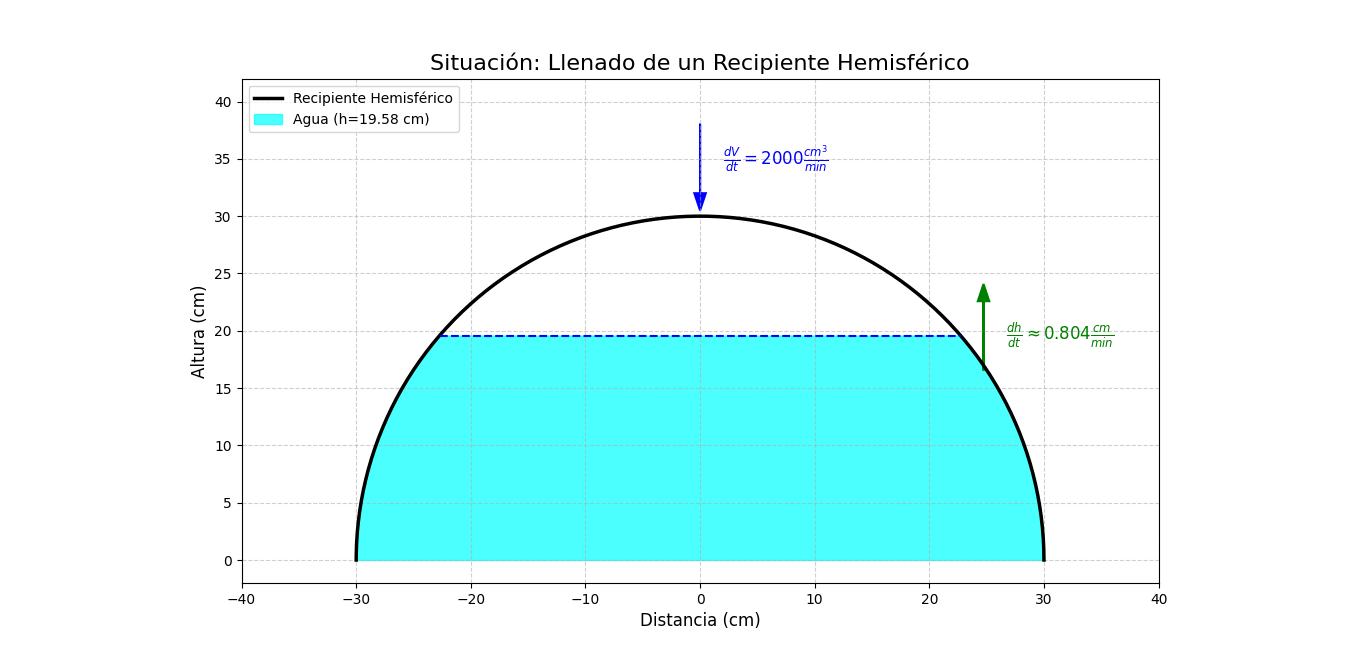
\includegraphics[width=1.2\textwidth]{Figure_3.png}
    \caption{Recipiente hemisférico}
    \label{fig:Figure_2}
\end{figure}
\section*{4.}
\section*{Análisis de la Función $f(\theta) = 2\cos\theta + \cos^2\theta$}
Analizaremos la función $f(\theta) = 2\cos\theta + \cos^2\theta$ en el intervalo cerrado $[0, \pi/2]$.

\section*{a) Intervalos de Crecimiento y Decrecimiento}

Para determinar dónde la función crece o decrece, necesitamos encontrar la primera derivada, $f'(\theta)$.

\paragraph{Cálculo de la primera derivada:}
Usando la regla de la cadena, obtenemos:
\begin{align*}
f'(\theta) &= \frac{d}{d\theta}(2\cos\theta + (\cos\theta)^2) \\
&= -2\sin\theta + 2(\cos\theta)(-\sin\theta) \\
&= -2\sin\theta - 2\sin\theta\cos\theta
\end{align*}
Factorizamos $-2\sin\theta$ para simplificar el análisis:
$$ f'(\theta) = -2\sin\theta(1 + \cos\theta) $$

\paragraph{Búsqueda de puntos críticos:}
Los puntos críticos ocurren cuando $f'(\theta) = 0$ o no está definida. La función está definida en todo el intervalo.
$$ -2\sin\theta(1 + \cos\theta) = 0 $$
Esto implica que:
\begin{itemize}
    \item $\sin\theta = 0 \implies \theta = 0$ en nuestro intervalo $[0, \pi/2]$.
    \item $1 + \cos\theta = 0 \implies \cos\theta = -1$, lo cual no tiene solución en $[0, \pi/2]$.
\end{itemize}
El único punto crítico se encuentra en el extremo del intervalo, en $\theta = 0$.

\paragraph{Análisis de signos de $f'(\theta)$:}
Para analizar el comportamiento de la función, evaluamos el signo de $f'(\theta)$ en el interior del intervalo, por ejemplo en $(0, \pi/2)$.
\begin{itemize}
    \item En $(0, \pi/2)$, el término $\sin\theta$ es siempre positivo.
    \item En $(0, \pi/2)$, el término $\cos\theta$ es siempre positivo, por lo que $(1 + \cos\theta)$ también es positivo.
\end{itemize}
Por lo tanto, el signo de $f'(\theta) = -2(\text{positivo})(\text{positivo})$ es siempre negativo en $(0, \pi/2)$.

\paragraph{Conclusión:}
Como $f'(\theta) < 0$ para todo $\theta \in (0, \pi/2)$, la función es estrictamente decreciente en todo el intervalo.
\begin{itemize}
    \item \textbf{Intervalo donde decrece:} $[0, \pi/2]$
    \item \textbf{Intervalo donde crece:} Ninguno.
\end{itemize}


\section*{b) Valores Máximos y Mínimos Locales}
Dado que la función es continua y monótonamente decreciente en el intervalo cerrado $[0, \pi/2]$, los valores extremos absolutos (y únicos) se encontrarán en los extremos del intervalo.

\begin{itemize}
    \item El \textbf{valor máximo} ocurre en $\theta = 0$:
    $$ f(0) = 2\cos(0) + \cos^2(0) = 2(1) + (1)^2 = 3 $$
    \item El \textbf{valor mínimo} ocurre en $\theta = \pi/2$:
    $$ f(\pi/2) = 2\cos(\pi/2) + \cos^2(\pi/2) = 2(0) + (0)^2 = 0 $$
\end{itemize}
No existen máximos o mínimos locales en el interior del intervalo.

\section*{c) Intervalos de Concavidad y Puntos de Inflexión}
Para el análisis de concavidad, calculamos la segunda derivada, $f''(\theta)$.

\paragraph{Cálculo de la segunda derivada:}
Partimos de $f'(\theta) = -2\sin\theta - 2\sin\theta\cos\theta = -2\sin\theta - \sin(2\theta)$.
\begin{align*}
f''(\theta) &= \frac{d}{d\theta}(-2\sin\theta - \sin(2\theta)) \\
&= -2\cos\theta - \cos(2\theta) \cdot 2 \\
&= -2\cos\theta - 2\cos(2\theta)
\end{align*}
Usamos la identidad del ángulo doble $\cos(2\theta) = 2\cos^2\theta - 1$:
$$ f''(\theta) = -2\cos\theta - 2(2\cos^2\theta - 1) = -4\cos^2\theta - 2\cos\theta + 2 $$

\paragraph{Búsqueda de posibles puntos de inflexión:}
Igualamos $f''(\theta)$ a cero:
$$ -4\cos^2\theta - 2\cos\theta + 2 = 0 $$
Dividimos por -2:
$$ 2\cos^2\theta + \cos\theta - 1 = 0 $$
Sea $u = \cos\theta$. La ecuación se convierte en $2u^2 + u - 1 = 0$, que se factoriza como $(2u-1)(u+1) = 0$. Las soluciones son $u = 1/2$ y $u = -1$.
\begin{itemize}
    \item $\cos\theta = 1/2 \implies \theta = \pi/3$ en nuestro intervalo.
    \item $\cos\theta = -1$, que no tiene solución en nuestro intervalo.
\end{itemize}
El único posible punto de inflexión es $\theta = \pi/3$.

\paragraph{Análisis de signos de $f''(\theta)$:}
Analizamos la concavidad en los intervalos $[0, \pi/3)$ y $(\pi/3, \pi/2]$.
\begin{itemize}
    \item Para $\theta \in [0, \pi/3)$, $\cos\theta > 1/2$. Tomemos $\theta = \pi/4$:
    $f''(\pi/4) = -4\cos^2(\pi/4) - 2\cos(\pi/4) + 2 = -4(1/2) - 2(\sqrt{2}/2) + 2 = -\sqrt{2} < 0$.
    La función es \textbf{cóncava hacia abajo}.
    \item Para $\theta \in (\pi/3, \pi/2]$, $\cos\theta < 1/2$. Tomemos $\theta = \pi/2$:
    $f''(\pi/2) = -4(0)^2 - 2(0) + 2 = 2 > 0$.
    La función es \textbf{cóncava hacia arriba}.
\end{itemize}

\paragraph{Conclusión:}
\begin{itemize}
    \item \textbf{Intervalo cóncavo hacia abajo:} $[0, \pi/3]$
    \item \textbf{Intervalo cóncavo hacia arriba:} $[\pi/3, \pi/2]$
    \item Como la concavidad cambia en $\theta = \pi/3$, hay un \textbf{punto de inflexión}.
    Calculamos su coordenada y:
    $$ f(\pi/3) = 2\cos(\pi/3) + \cos^2(\pi/3) = 2(1/2) + (1/2)^2 = 1 + 1/4 = 5/4 $$
    El punto de inflexión es \textbf{$(\pi/3, 5/4)$}.
\end{itemize}

\section*{d) Gráfica de la Función}
Para visualizar la función $f(\theta) = 2\cos\theta + \cos$

\begin{figure}[h!]
    \centering
    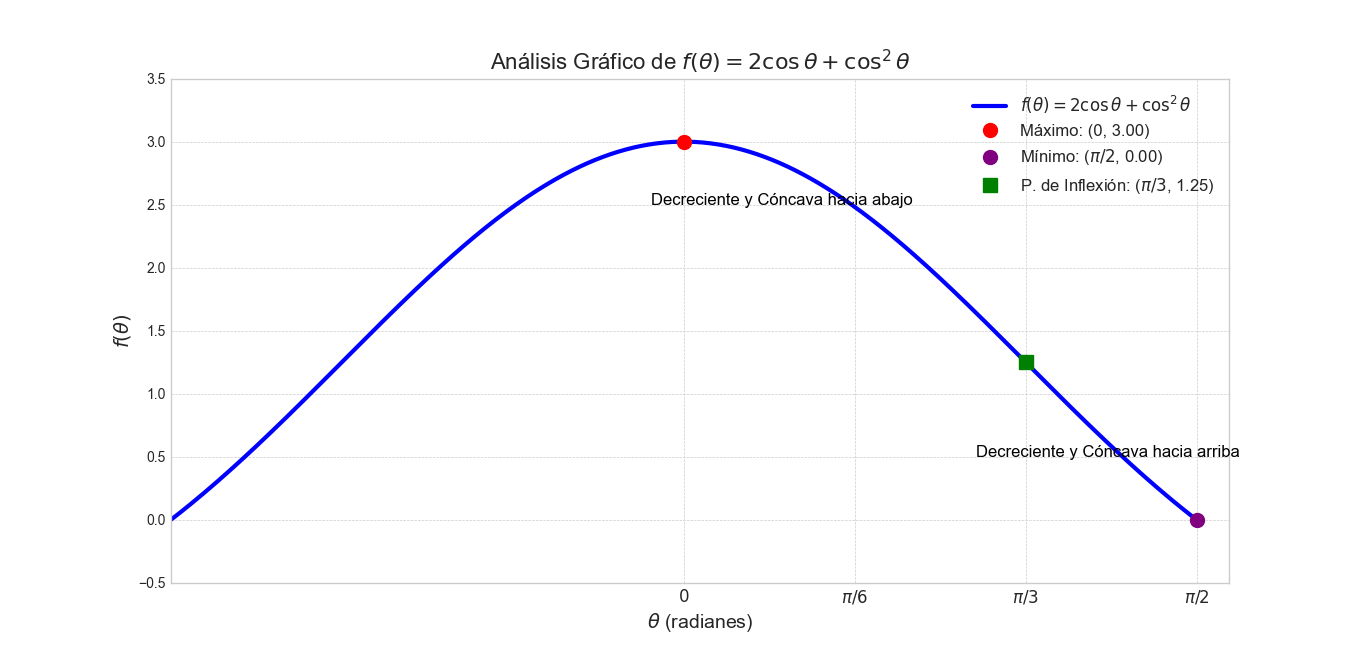
\includegraphics[width=1\textwidth]{Figure_4.png}
    \caption{Análisis Gráfica}
    \label{fig:Figure_2}
\end{figure}
\section*{5.}
\section*{a. Análisis de $f(x) = \frac{2x^2}{x^2-1}$}
\begin{enumerate}
    \item[\textbf{A.}] \textbf{Dominio:} La función no está definida cuando el denominador es cero, es decir, $x^2-1=0 \implies x=\pm1$.
    \[ D_f = \{x \in \mathbb{R} | x \neq \pm 1\} = (-\infty, -1) \cup (-1, 1) \cup (1, \infty) \]

    \item[\textbf{B.}] \textbf{Intersecciones:}
    \begin{itemize}
        \item \textbf{Eje y:} $f(0) = \frac{2(0)^2}{0^2-1} = 0$. El punto es $(0,0)$.
        \item \textbf{Eje x:} $f(x) = 0 \implies 2x^2 = 0 \implies x=0$. El punto es $(0,0)$.
    \end{itemize}

    \item[\textbf{C.}] \textbf{Simetría:} $f(-x) = \frac{2(-x)^2}{(-x)^2-1} = \frac{2x^2}{x^2-1} = f(x)$. La función es \textbf{par} y simétrica respecto al eje y.

    \item[\textbf{D.}] \textbf{Asíntotas:}
    \begin{itemize}
        \item \textbf{Horizontales:} $\lim_{x\to\pm\infty} \frac{2x^2}{x^2-1} = \lim_{x\to\pm\infty} \frac{2}{1 - 1/x^2} = 2$. La asíntota horizontal es $y=2$.
        \item \textbf{Verticales:} En $x=1$ y $x=-1$.
        $$ \lim_{x\to1^+} f(x) = \infty, \quad \lim_{x\to1^-} f(x) = -\infty $$
        $$ \lim_{x\to-1^+} f(x) = -\infty, \quad \lim_{x\to-1^-} f(x) = \infty $$
    \end{itemize}

    \item[\textbf{E.}] \textbf{Crecimiento y Decrecimiento:}
    $$ f'(x) = \frac{4x(x^2-1) - 2x^2(2x)}{(x^2-1)^2} = \frac{-4x}{(x^2-1)^2} $$
    \begin{itemize}
        \item Creciente ($f'(x)>0$): $(-\infty, -1) \cup (-1, 0)$.
        \item Decreciente ($f'(x)<0$): $(0, 1) \cup (1, \infty)$.
    \end{itemize}

    \item[\textbf{F.}] \textbf{Extremos Locales:} El único número crítico es $x=0$. Como $f'$ cambia de $+$ a $-$ en $x=0$, hay un \textbf{máximo local} en el punto $(0, f(0)) = (0,0)$.

    \item[\textbf{G.}] \textbf{Concavidad:}
    $$ f''(x) = \frac{-4(x^2-1)^2 - (-4x) \cdot 2(x^2-1)(2x)}{(x^2-1)^4} = \frac{12x^2+4}{(x^2-1)^3} $$
    \begin{itemize}
        \item Cóncava hacia arriba ($f''(x)>0$): $(-\infty, -1) \cup (1, \infty)$.
        \item Cóncava hacia abajo ($f''(x)<0$): $(-1, 1)$.
    \end{itemize}
    No hay puntos de inflexión ya que $x=\pm1$ no están en el dominio.

    \item[\textbf{H.}] \textbf{Gráfica:} Se traza una curva simétrica al eje y con asíntotas en $y=2$, $x=1$ y $x=-1$. La curva pasa por $(0,0)$ como un máximo local, es creciente hasta $x=0$ y decreciente después, con la concavidad cambiando en las asíntotas verticales.
\end{enumerate}
\begin{figure}[ht]
    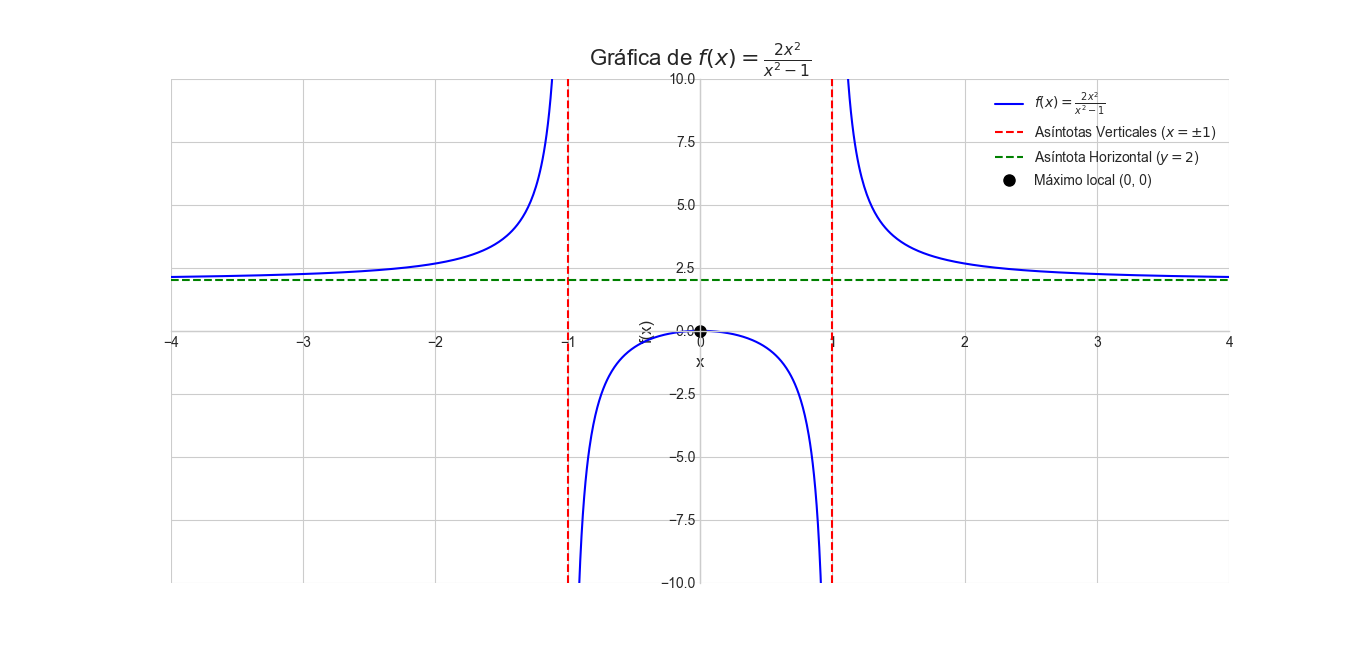
\includegraphics
    [width=1\textwidth]{Figure_9.png}
    \caption{Gráfica de $f(x) = \frac{2x^2}{x^2-1}$}
    \label{fig:Figure_1}
\end{figure}
\newpage
\section*{b. Análisis de $f(x) = xe^x$}
\begin{enumerate}
    \item[\textbf{A.}] \textbf{Dominio:} $D_f = \mathbb{R}$.

    \item[\textbf{B.}] \textbf{Intersecciones:} $f(x)=0 \implies xe^x = 0 \implies x=0$. La única intersección es en el origen, $(0,0)$.

    \item[\textbf{C.}] \textbf{Simetría:} La función no es par ni impar.

    \item[\textbf{D.}] \textbf{Asíntotas:}
    \begin{itemize}
        \item $\lim_{x\to\infty} xe^x = \infty$. No hay asíntota horizontal a la derecha.
        \item $\lim_{x\to-\infty} xe^x = \lim_{x\to-\infty} \frac{x}{e^{-x}} \overset{L'H}{=} \lim_{x\to-\infty} \frac{1}{-e^{-x}} = 0$. La asíntota horizontal es $y=0$ (a la izquierda).
    \end{itemize}

    \item[\textbf{E.}] \textbf{Crecimiento y Decrecimiento:}
    $$ f'(x) = 1 \cdot e^x + x \cdot e^x = (x+1)e^x $$
    \begin{itemize}
        \item Creciente ($f'(x)>0$): $(-1, \infty)$.
        \item Decreciente ($f'(x)<0$): $(-\infty, -1)$.
    \end{itemize}

    \item[\textbf{F.}] \textbf{Extremos Locales:} El número crítico es $x=-1$. Como $f'$ cambia de $-$ a $+$ en $x=-1$, hay un \textbf{mínimo local (y absoluto)} en el punto $(-1, f(-1)) = (-1, -e^{-1})$. Punto exacto: $(-1, -1/e)$.

    \item[\textbf{G.}] \textbf{Concavidad:}
    $$ f''(x) = 1 \cdot e^x + (x+1)e^x = (x+2)e^x $$
    \begin{itemize}
        \item Cóncava hacia arriba ($f''(x)>0$): $(-2, \infty)$.
        \item Cóncava hacia abajo ($f''(x)<0$): $(-\infty, -2)$.
    \end{itemize}
    Hay un cambio de concavidad en $x=-2$. El \textbf{punto de inflexión} es $(-2, f(-2)) = (-2, -2e^{-2})$. Punto exacto: $(-2, -2/e^2)$.

    \item[\textbf{H.}] \textbf{Gráfica:} La curva viene desde la asíntota $y=0$ a la izquierda, decrece hasta el mínimo en $(-1, -1/e)$, y luego crece indefinidamente. La concavidad cambia de hacia abajo a hacia arriba en el punto de inflexión $(-2, -2/e^2)$.
\end{enumerate}
\begin{figure}[ht]
    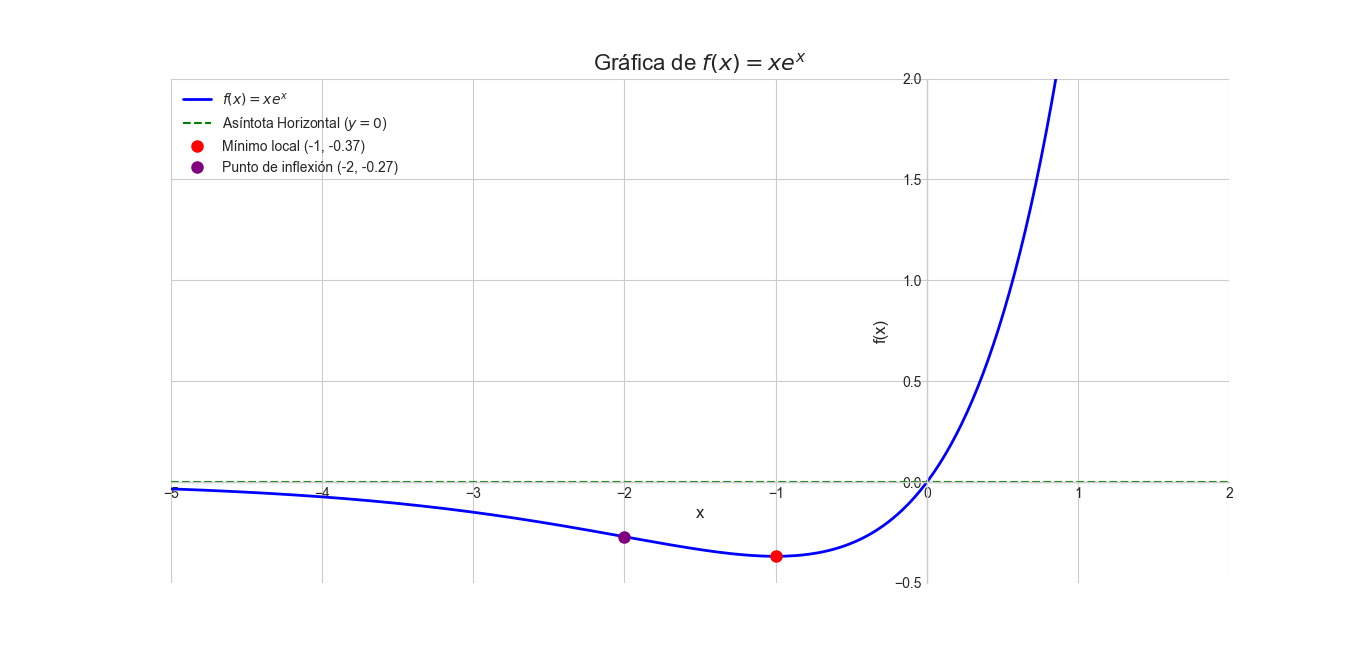
\includegraphics
    [width=1\textwidth]{Figure_10.png}
    \caption{Gráfica de $f(x) = xe^x$}
    \label{fig:Figure_1}
\end{figure}
\newpage

\section*{c. Análisis de $f(x) = \ln(4-x^2)$}
\begin{enumerate}
    \item[\textbf{A.}] \textbf{Dominio:} Se necesita $4-x^2 > 0 \implies x^2 < 4 \implies |x| < 2$.
    $$ D_f = (-2, 2) $$

    \item[\textbf{B.}] \textbf{Intersecciones:}
    \begin{itemize}
        \item \textbf{Eje y:} $f(0) = \ln(4)$. Punto exacto: $(0, \ln(4))$.
        \item \textbf{Eje x:} $\ln(4-x^2) = 0 \implies 4-x^2 = 1 \implies x^2 = 3 \implies x = \pm\sqrt{3}$. Puntos exactos: $(\sqrt{3}, 0)$ y $(-\sqrt{3}, 0)$.
    \end{itemize}
    
    \item[\textbf{C.}] \textbf{Simetría:} $f(-x) = \ln(4-(-x)^2) = \ln(4-x^2) = f(x)$. La función es \textbf{par} y simétrica respecto al eje y.

    \item[\textbf{D.}] \textbf{Asíntotas:}
    \begin{itemize}
        \item \textbf{Verticales:} En los extremos del dominio, $x=2$ y $x=-2$.
        $$ \lim_{x\to2^-} \ln(4-x^2) = -\infty, \quad \lim_{x\to-2^+} \ln(4-x^2) = -\infty $$
    \end{itemize}

    \item[\textbf{E.}] \textbf{Crecimiento y Decrecimiento:}
    $$ f'(x) = \frac{-2x}{4-x^2} $$
    \begin{itemize}
        \item Creciente ($f'(x)>0$): $(-2, 0)$.
        \item Decreciente ($f'(x)<0$): $(0, 2)$.
    \end{itemize}

    \item[\textbf{F.}] \textbf{Extremos Locales:} El número crítico es $x=0$. Como $f'$ cambia de $+$ a $-$ en $x=0$, hay un \textbf{máximo local} en el punto $(0, f(0))$. Punto exacto: $(0, \ln(4))$.

    \item[\textbf{G.}] \textbf{Concavidad:}
    $$ f''(x) = \frac{-2(4-x^2) - (-2x)(-2x)}{(4-x^2)^2} = \frac{-8-2x^2}{(4-x^2)^2} = \frac{-2(4+x^2)}{(4-x^2)^2} $$
    Como $f''(x) < 0$ para todo $x$ en el dominio, la función es siempre \textbf{cóncava hacia abajo} en $(-2, 2)$. No hay puntos de inflexión.

    \item[\textbf{H.}] \textbf{Gráfica:} La curva es una forma de campana invertida, simétrica respecto al eje y. Está contenida entre sus asíntotas verticales $x=-2$ y $x=2$. Alcanza su punto más alto en el máximo local $(0, \ln(4))$ y cruza el eje x en $\pm\sqrt{3}$.
\end{enumerate}
\begin{figure}[ht]
    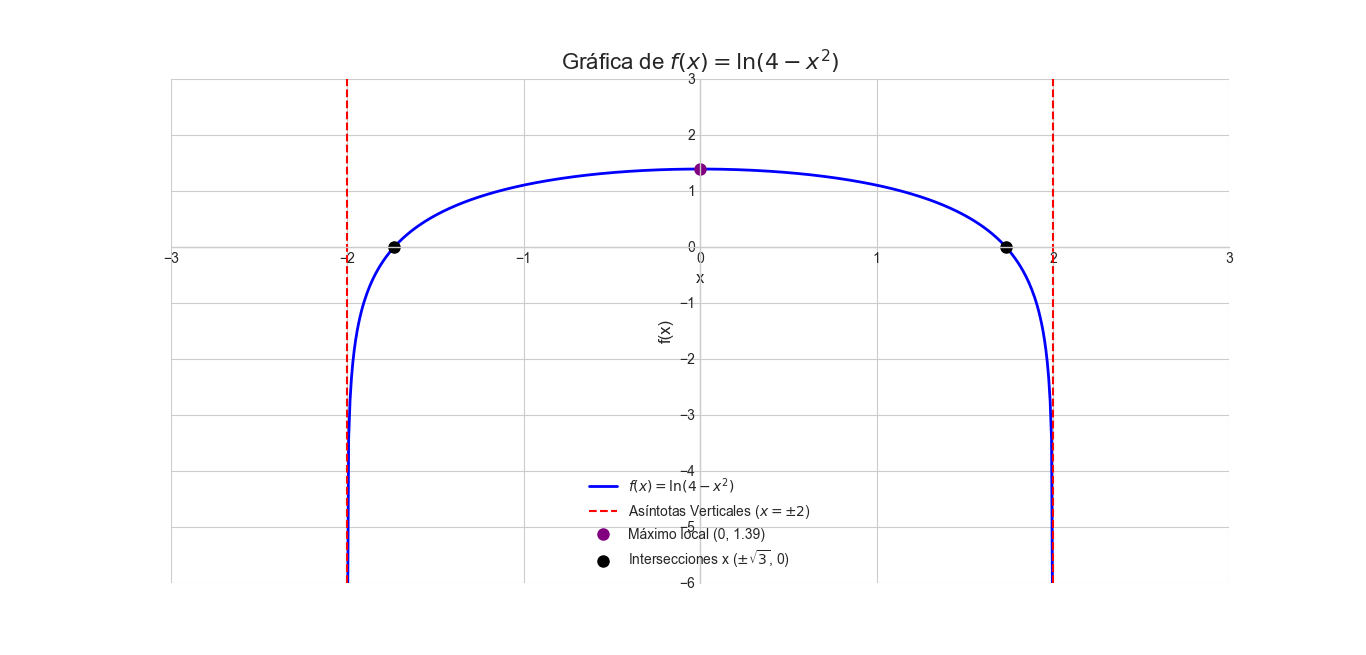
\includegraphics
    [width=1\textwidth]{Figure_11.png}
    \caption{Gráfica de $f(x) = \ln(4-x^2)$}
    \label{fig:Figure_1}
\end{figure}
\newpage
\section*{6.}
\section*{Caso 1: Contenedor sin Tapa}
Se busca minimizar el costo de los materiales para un contenedor rectangular con un volumen fijo de 10 m³. Se analizarán dos escenarios: uno sin tapa y otro con tapa, para luego comparar los resultados.



\subsection*{Planteamiento de Ecuaciones}
Sean $w$ el ancho, $l$ el largo y $h$ la altura del contenedor.
\begin{itemize}
    \item \textbf{Relación de la base:} $l = 2w$.
    \item \textbf{Restricción de Volumen (V):} $V = lwh = 10$.
\end{itemize}
Sustituyendo la relación de la base en el volumen, obtenemos:
$$ (2w)(w)h = 10 \implies 2w^2h = 10 $$
De aquí, podemos expresar la altura $h$ en función del ancho $w$:
$$ h = \frac{10}{2w^2} = \frac{5}{w^2} $$

\subsection*{Función de Costo}
El costo total ($C$) es la suma del costo de la base y el costo de los cuatro costados.
\begin{itemize}
    \item \textbf{Área de la base:} $A_{\text{base}} = lw = (2w)w = 2w^2$.
    \item \textbf{Costo de la base:} $C_{\text{base}} = (10 \$/\text{m}^2) \cdot (2w^2 \text{ m}^2) = 20w^2 \$$.
    \item \textbf{Área de los costados:} $A_{\text{costados}} = 2(wh) + 2(lh) = 2wh + 2(2w)h = 6wh$.
    \item \textbf{Costo de los costados:} $C_{\text{costados}} = (6 \$/\text{m}^2) \cdot (6w \cdot h \text{ m}^2) = 36w \cdot h \$$.
\end{itemize}
La función de costo total es $C(w,h) = 20w^2 + 36wh$. Sustituimos $h = 5/w^2$ para obtener una función de una sola variable:
$$ C(w) = 20w^2 + 36w\left(\frac{5}{w^2}\right) = 20w^2 + \frac{180}{w} $$

\subsection*{Optimización por Cálculo}
Para encontrar el costo mínimo, derivamos $C(w)$ e igualamos a cero.
$$ C'(w) = \frac{d}{dw}\left(20w^2 + 180w^{-1}\right) = 40w - 180w^{-2} = 40w - \frac{180}{w^2} $$
Igualando a cero:
$$ 40w - \frac{180}{w^2} = 0 \implies 40w^3 = 180 \implies w^3 = 4.5 $$
$$ w = \sqrt[3]{4.5} \approx 1.651 \text{ m} $$
La segunda derivada, $C''(w) = 40 + 360/w^3$, es siempre positiva para $w>0$, lo que confirma que este punto es un mínimo.

\subsection*{Resultados del Caso 1}
Las dimensiones óptimas son:
\begin{itemize}
    \item Ancho: $w \approx 1.651$ m.
    \item Largo: $l = 2w \approx 3.302$ m.
    \item Altura: $h = 5/w^2 \approx 1.834$ m.
\end{itemize}
El costo mínimo es: $C(1.651) = 20(1.651)^2 + \frac{180}{1.651} \approx \textbf{\$163.54}$.

\newpage

\section*{Caso 2: Contenedor con Tapa}

\subsection*{Función de Costo}
Se añade el costo de una tapa fabricada con el material de los lados (\$6/m²).
\begin{itemize}
    \item \textbf{Área de la tapa:} $A_{\text{tapa}} = lw = 2w^2$.
    \item \textbf{Costo de la tapa:} $C_{\text{tapa}} = (6 \$/\text{m}^2) \cdot (2w^2 \text{ m}^2) = 12w^2 \$$.
\end{itemize}
La nueva función de costo total $C_t(w)$ es:
$$ C_t(w) = (\text{Costo sin tapa}) + (\text{Costo de la tapa}) = \left(20w^2 + \frac{180}{w}\right) + 12w^2 $$
$$ C_t(w) = 32w^2 + \frac{180}{w} $$

\subsection*{Optimización por Cálculo}
Derivamos la nueva función $C_t(w)$ e igualamos a cero:
$$ C_t'(w) = 64w - \frac{180}{w^2} $$
$$ 64w - \frac{180}{w^2} = 0 \implies 64w^3 = 180 \implies w^3 = \frac{180}{64} = 2.8125 $$
$$ w = \sqrt[3]{2.8125} \approx 1.412 \text{ m} $$
La segunda derivada $C_t''(w) = 64 + 360/w^3$ también es siempre positiva.

\subsection*{Resultados del Caso 2}
Las nuevas dimensiones óptimas son:
\begin{itemize}
    \item Ancho: $w \approx 1.412$ m.
    \item Largo: $l = 2w \approx 2.824$ m.
    \item Altura: $h = 5/w^2 \approx 2.505$ m.
\end{itemize}
El costo mínimo es: $C_t(1.412) = 32(1.412)^2 + \frac{180}{1.412} \approx \textbf{\$191.30}$.

\section*{Justificación y Comparación Final}

\subsection*{Respuesta a la Pregunta}
No, el costo de los materiales que hacen más barato el contenedor \textbf{no es el mismo} en ambos escenarios. Los cálculos demuestran que el costo mínimo y las dimensiones óptimas cambian al añadir la tapa.

\subsection*{Tabla Comparativa}
\begin{center}
\begin{tabular}{|l|c|c|}
\hline
\textbf{Característica} & \textbf{Contenedor sin Tapa} & \textbf{Contenedor con Tapa} \\
\hline
Ancho ($w$) & $\approx 1.651$ m & $\approx 1.412$ m \\
Largo ($l$) & $\approx 3.302$ m & $\approx 2.824$ m \\
Altura ($h$) & $\approx 1.834$ m & $\approx 2.505$ m \\
\hline
\textbf{Costo Mínimo} & \textbf{\$163.54} & \textbf{\$191.30} \\
\hline
\end{tabular}
\end{center}

\subsection*{Justificación}
Las dimensiones cambian porque la función de costo se modifica. En el segundo caso, el costo total de las superficies horizontales (base a \$10/m² y tapa a \$6/m²) tiene un mayor peso relativo en el costo total. Para minimizarlo, el diseño óptimo reduce el área de estas superficies (disminuyendo $w$ y $l$) y compensa el volumen perdido aumentando la altura $h$.

\begin{figure}[h!]
    \centering
    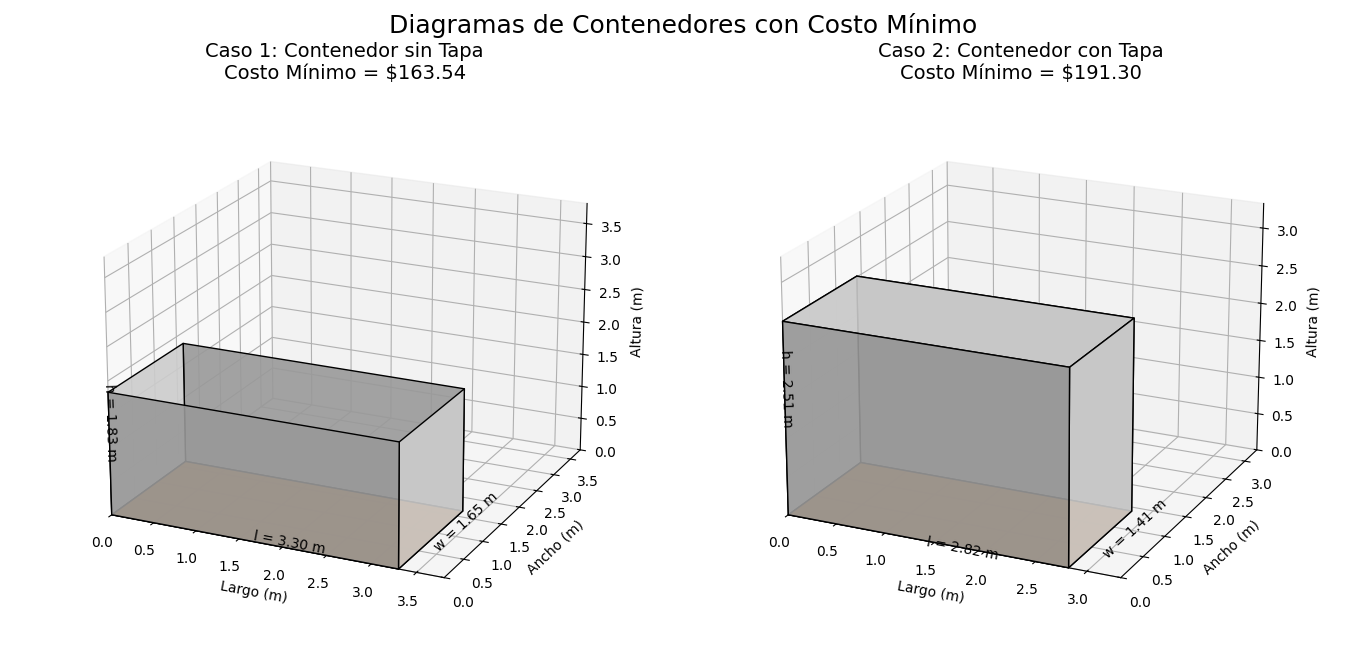
\includegraphics[width=1\textwidth]{Figure_5.png}
    \caption{Diagramas de contenedores}
    \label{fig:Figure_2}
\end{figure}
\section*{7.}
\section*{Optimización: Volumen Máximo de un Cilindro en una Esfera}

Se busca encontrar las dimensiones del cilindro de mayor volumen posible que puede ser inscrito en una esfera de radio constante $r$.

Sean $x$ el radio del cilindro y $h$ su altura. El volumen del cilindro, que deseamos maximizar, es:
$$ V = \pi x^2 h $$
Esta función depende de dos variables, $x$ y $h$. Necesitamos una ecuación de restricción para relacionarlas.


Al observar un corte transversal, se forma un triángulo rectángulo con el centro de la esfera, un punto en el borde de la base del cilindro y el centro de la base del cilindro. Los lados de este triángulo son:
\begin{itemize}
    \item Hipotenusa: El radio de la esfera, $r$.
    \item Un cateto: El radio del cilindro, $x$.
    \item Otro cateto: La mitad de la altura del cilindro, $h/2$.
\end{itemize}

\section*{2. Ecuación de Restricción}
Aplicando el Teorema de Pitágoras a este triángulo, obtenemos nuestra ecuación de restricción:
$$ x^2 + \left(\frac{h}{2}\right)^2 = r^2 \implies x^2 + \frac{h^2}{4} = r^2 $$
De esta ecuación, es conveniente despejar $x^2$:
$$ x^2 = r^2 - \frac{h^2}{4} $$

\section*{3. Optimización de la Función de Volumen}
Sustituimos la expresión para $x^2$ en la fórmula del volumen para obtener una función de una sola variable, $h$:
$$ V(h) = \pi \left(r^2 - \frac{h^2}{4}\right) h = \pi \left(r^2h - \frac{h^3}{4}\right) $$
El dominio físico para la altura es $0 < h < 2r$. Para encontrar el volumen máximo, derivamos $V(h)$ con respecto a $h$ e igualamos a cero.
$$ V'(h) = \frac{d}{dh} \left[ \pi \left(r^2h - \frac{h^3}{4}\right) \right] = \pi \left(r^2 - \frac{3h^2}{4}\right) $$
Igualando a cero para encontrar los puntos críticos:
$$ \pi \left(r^2 - \frac{3h^2}{4}\right) = 0 \implies r^2 = \frac{3h^2}{4} $$
$$ 4r^2 = 3h^2 \implies h^2 = \frac{4r^2}{3} \implies h = \sqrt{\frac{4r^2}{3}} = \frac{2r}{\sqrt{3}} = \frac{2\sqrt{3}r}{3} $$
Para verificar que este valor corresponde a un máximo, usamos el criterio de la segunda derivada:
$$ V''(h) = \frac{d}{dh} \left[ \pi \left(r^2 - \frac{3h^2}{4}\right) \right] = \pi \left(-\frac{6h}{4}\right) = -\frac{3\pi h}{2} $$
Como $h$ es una altura, $h>0$, por lo que $V''(h)$ es siempre negativa. Esto confirma que hemos encontrado un máximo.

\section*{4. Conclusión y Resultados}
Hemos encontrado la altura óptima del cilindro. Ahora encontramos el radio óptimo $x$ usando la ecuación de restricción:
$$ x^2 = r^2 - \frac{h^2}{4} = r^2 - \frac{1}{4}\left(\frac{4r^2}{3}\right) = r^2 - \frac{r^2}{3} = \frac{2r^2}{3} $$
$$ x = \sqrt{\frac{2r^2}{3}} = \frac{\sqrt{2}r}{\sqrt{3}} = \frac{\sqrt{6}r}{3} $$
Finalmente, el volumen máximo es:
$$ V_{\text{max}} = \pi x^2 h = \pi \left(\frac{2r^2}{3}\right) \left(\frac{2r}{\sqrt{3}}\right) = \frac{4\pi r^3}{3\sqrt{3}} = \frac{4\sqrt{3}\pi r^3}{9} $$

\vspace{0.5cm}

\textbf{Resumen de las dimensiones del cilindro de volumen máximo:}
\begin{itemize}
    \item \textbf{Altura:} $h = \frac{2\sqrt{3}r}{3}$
    \item \textbf{Radio:} $x = \frac{\sqrt{6}r}{3}$
    \item \textbf{Volumen Máximo:} $V = \frac{4\sqrt{3}\pi r^3}{9}$
\end{itemize}

\begin{figure}[h!]
    \centering
    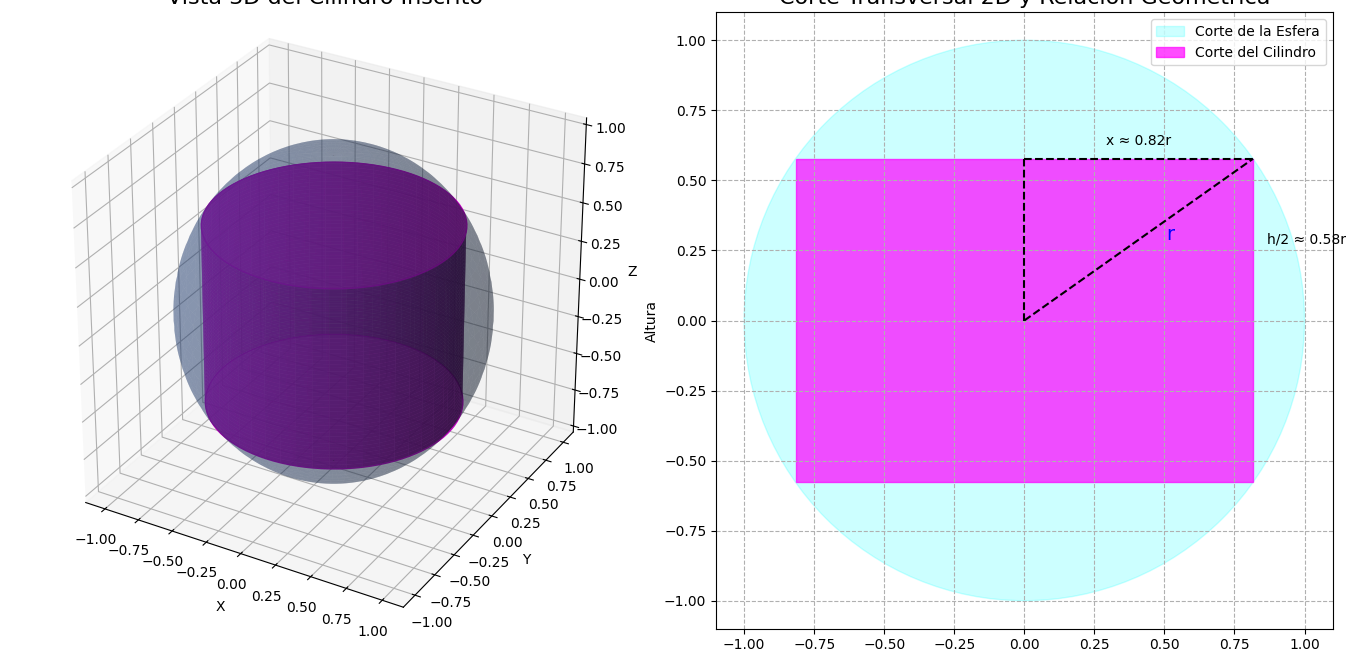
\includegraphics[width=0.8\textwidth]{Figure_7.png}
    \caption{Cilindro y esfera}
    \label{fig:Figure_2}
\end{figure}

\begin{thebibliography}{9}
\bibitem{stewart8} Stewart, J. (2016). \textit{Cálculo de una variable: Trascendentes tempranas}. 8va edición. Cengage Learning.
\end{thebibliography}

\end{document}